% ============================================================
%  ICRefine — Results section  (NeurIPS 2026 format)
%
%  To compile:
%    1. Copy neurips_2026.sty from
%         Formatting_Instructions_For_NeurIPS_2026 (1)/neurips_2026.sty
%       into this directory, then run:
%         pdflatex findings_draft.tex
%    OR compile directly from the formatting-instructions folder.
% ============================================================

\documentclass{article}

% ── NeurIPS 2026 style ──────────────────────────────────────
\usepackage{neurips_2026}   % submission (anonymous, line-numbered)
% \usepackage[preprint]{neurips_2026}  % arXiv preprint

% ── Standard NeurIPS package set ────────────────────────────
\usepackage[utf8]{inputenc}
\usepackage[T1]{fontenc}
\usepackage{hyperref}
\usepackage{url}
\usepackage{booktabs}
\usepackage{amsfonts}
\usepackage{amsmath}
\usepackage{nicefrac}
\usepackage{microtype}
\usepackage{xcolor}

% ── Additional packages (figures, tables, code) ─────────────
\usepackage{graphicx}
\usepackage{subcaption}
\usepackage{multirow}
\usepackage{array}
\usepackage{listings}
\usepackage{enumitem}

% ── Figure search path ──────────────────────────────────────
\graphicspath{{./figures/}}

% ── Code / cheatsheet example style ─────────────────────────
\definecolor{codebackground}{gray}{0.95}
\lstset{
  backgroundcolor  = \color{codebackground},
  basicstyle       = \ttfamily\footnotesize,
  frame            = single,
  framesep         = 4pt,
  rulecolor        = \color{gray!50},
  breaklines       = true,
  captionpos       = b,
  aboveskip        = 6pt,
  belowskip        = 6pt,
  xleftmargin      = 4pt,
  xrightmargin     = 4pt,
}

% ============================================================
\title{ICRefine: Iterative Cheatsheet Refinement for In-Context Learning}

\author{%
  Anonymous Author(s)
}

\begin{document}
\maketitle

% ============================================================
\section{Method}
\label{sec:method}
% ============================================================

\subsection{Cheatsheet format}
\label{sec:format}

\textsc{ICRefine} produces a \emph{cheatsheet} consisting of two components, both prepended
to the inference prompt.
The \textbf{prior knowledge (PK)} is a free-form natural-language ruleset
($\leq$12\,000 characters) encoding general task heuristics.
\textbf{Case studies} follow a structured \texttt{ACTIVATE~IF / WHY} format:
each case study specifies a set of trigger conditions (structural predicates over the input),
a correction rationale, and annotated support examples
(see Listing~\ref{lst:gs_cs} in Section~\ref{sec:overfitting} for a concrete example).
At inference time, the full cheatsheet is prepended verbatim to each test prompt; the model
applies relevant case studies alongside the PK rules when generating its answer.

\subsection{Phase 0: bootstrap}
\label{sec:phase0}

The pipeline initialises the PK by prompting the train model with the first
$n_\text{boot}=75$ training examples and requesting a concise rules-and-heuristics summary
(single pass, no iteration).
Phase~0 follows the cheatsheet generation style of \citet{csicl2024}, with the
train model (gpt-4.1-mini) in place of the full gpt-4.1 used by both their baseline
and ours (see Section~\ref{sec:eval}).

\subsection{Phase 1: prior-knowledge patching}
\label{sec:phase1}

Phase~1 iteratively revises the PK using a sample-and-accept loop.
At each iteration:

\begin{enumerate}[noitemsep,topsep=2pt]
  \item Score all 100 training items against the current PK; collect failures $\mathcal{F}_t$.
  \item Sample $\min(15,|\mathcal{F}_t|)$ failures; optionally append gold chain-of-thought
        (\texttt{item["reason"]}, oracle injection) as a ``Correct reasoning'' contrast block.
  \item Generate one candidate PK revision (temperature 0.3).
  \item Apply two acceptance gates in sequence:
        \textbf{(a) fix-rate gate}: re-score the 15 shown failures; accept if
        $\text{fix\_rate} \geq 0.20$;
        \textbf{(b) regression gate}: sample $\min(40, |\mathcal{C}_t|)$ currently-correct
        items; accept if $\text{regress\_rate} \leq 0.20$.
  \item If both gates pass, replace the PK and re-score the full training set.
\end{enumerate}

Phase~1 exits when: training accuracy $\geq 0.85$, two consecutive iterations produce no
accepted patch, or 4 iterations are exhausted.
The 4-iteration cap is motivated by API cost: on the tasks studied here, most of the
Phase~1 gain arrives in the first two accepted patches; iterations 3--4 rarely move
accuracy more than 1--2\,pp.
Relaxing the cap is a direction for future work.

\subsection{Phase 2: partition-based case study generation}
\label{sec:phase2}

Phase~2 partitions remaining training failures by structural error type, then generates one
case study per non-trivial partition.
Partitions are computed deterministically from item-level structural features (no LLM
involvement); only partitions with $\geq 3$ failures are processed.
For each active partition:

\begin{enumerate}[noitemsep,topsep=2pt]
  \item Generate $N=3$ candidate case studies in parallel at temperatures
        $[0.3,\,0.6,\,0.9]$.
        Each candidate is conditioned on the partition's failure set, the current cheatsheet,
        and (optionally) oracle context.
        Structural \texttt{ACTIVATE~IF} predicates derived from the partition key are
        prepended to every candidate to guarantee correct-partition activation.
  \item Mini-evaluate all candidates against the partition's failure set; select the
        highest fix-rate candidate.
  \item Apply two acceptance gates:
        \textbf{(a) fix-rate gate}: accept if $\text{fix\_rate} \geq 0.30$;
        \textbf{(b) regression gate}: sample $\leq 50$ partition-matched correct items;
        accept if regression $\leq 0.15$.
  \item If both pass, add the case study to the cheatsheet; otherwise archive the candidate
        (up to 8 per partition) for re-evaluation in later iterations.
  \item Up to 3 generation attempts are made per partition per outer iteration;
        archived candidates are re-evaluated before each new attempt.
\end{enumerate}

Phase~2 exits when all partitions retire ($\leq 2$ failures remaining), two consecutive outer
iterations add no case study, or 5 outer iterations are exhausted.
When $\geq 3$ case studies exist, a similarity gate checks whether new candidates duplicate
or can be merged with existing ones before acceptance.

\subsection{Evolutionary Algorithm Phase~1}
\label{sec:ea_method}

Standard Phase~1 fails when the bootstrap PK already exceeds the 85\% accuracy goal,
applying zero patches.
To overcome this, the \textbf{EA Phase~1} variant replaces single-candidate search with
population-based exploration.

\paragraph{Population.}
Three members are maintained with distinct generation roles:
\emph{conservative} (temperature 0.2; targeted clarification edits),
\emph{generative} (temperature 0.7; unconstrained rewrites),
and \emph{structural} (temperature 0.3; explicit TIGHTEN/SPLIT/ADD\textunderscore GUARD
operations).
All members are scored on a fixed 80\%/20\% train/validation split;
only validation accuracy drives selection.

\paragraph{Per-generation loop.}
In generation 1, the failure set is partitioned disjointly across members so each sees a
distinct failure slice.
From generation 2 onward, each member samples $60\%$ of its own failures, rotated to
avoid repetition.
Candidates are accepted if they satisfy:
\textbf{(a) size}: $|\text{candidate}| \leq 12{,}000$ characters;
\textbf{(b) curriculum net-gain}: $n_\text{fixed} \geq \lambda(g) \cdot n_\text{regressed}$,
where $\lambda(g) = 1.0 + (g-1)/(G-1)$ ramps from 1.0 (loose, generation 1) to 2.0
(strict, final generation);
\textbf{(c) absolute regression cap}: $n_\text{regressed} \leq \max\!\left(3,\;
0.20 \cdot |\mathcal{C}_\text{pool}|\right)$.
Regression is measured on $\min(20,|\mathcal{C}_\text{own}|)$ own-correct items plus
$\min(10,|\mathcal{C}_\text{sib}|)$ items from each sibling's correct pool.

\paragraph{Survivor selection and crossover.}
After each generation, the top $k=2$ members by validation accuracy survive.
If $\geq 2$ survivors exist, a crossover step prompts the train model to merge them into a
child PK that inherits each survivor's unique wins while avoiding their shared failures
(temperature 0.3).
The child is scored and added to the population; the best-ever PK across all generations is
maintained as an elite and replaces the weakest member each generation.
The algorithm exits when all members are static for $\geq 2$ consecutive generations or
4 generations are exhausted.

\subsection{Oracle injection}
\label{sec:oracle_method}

When available, the gold chain-of-thought (\texttt{item["reason"]}) is injected into both
Phase~1 and Phase~2 prompts as a ``Correct reasoning'' contrast block alongside each failure.
The injection priority is: task-specific pre-computed oracle $>$ \texttt{item["reason"]}
dataset field $>$ external oracle CSV lookup.

Oracle injection was a \emph{default design choice} in the initial v3 pipeline, adopted
on the assumption that gold reasoning would help the train model identify better correction
rules.
It was not originally conceived as an experimental knob.
After observing that CJ transfer accuracy was substantially below the CS-ICL baseline
despite high training accuracy, we hypothesised oracle contamination as the cause:
oracle-assisted Phase~1 and Phase~2 prompts may produce rules that encode
the train model's oracle-assisted reasoning style rather than model-independent
correction patterns.
Experiment \textbf{E3} tests this hypothesis by disabling oracle injection for both phases
(\texttt{--no-phase1-oracle --no-phase2-oracle}); Section~\ref{sec:oracle} reports the
causal effect on transfer accuracy.

\subsection{Evaluation setup}
\label{sec:eval}

\paragraph{Reasoning-first (RF) scoring.}
All conditions are evaluated with \emph{reasoning-first} (RF) scoring: the model generates a
free-form chain-of-thought, then outputs \texttt{VERDICT:~(X)} as the final line.
RF scoring is motivated by a striking format artifact we observed in earlier CoT evaluations:
tasks such as web\_of\_lies scored 42--66\% under verdict-first CoT prompting
but 99--100\% under RF prompting---a gap of over 30\,pp driven entirely by prompt format,
not model capability or cheatsheet quality.
Because standard CoT evaluation conflates format sensitivity with model performance,
we use RF scoring throughout; all comparisons are therefore internally consistent
and free of this artifact.
Readers evaluating claims in the broader CoT-evaluation literature should note that
verdict-first scoring can produce similar format-induced gaps, and results reported
under different prompt formats may not be directly comparable.
We regard this format sensitivity as a noteworthy finding in its own right---it affects any
cheatsheet-ICL evaluation that uses verdict-first CoT scoring---and plan to report it with a
systematic comparison table in an appendix of the full submission.

\paragraph{Dataset.}
We use BIG-Bench Hard (BBH): 11 tasks, 100 training and 87--250 test examples per task.
Seven tasks reach $\geq 95\%$ accuracy after Phase~0 bootstrap alone and are excluded from
detailed analysis (boolean\_expressions, navigate, web\_of\_lies, logical\_deduction\_three,
sports\_understanding, formal\_fallacies on the train model, snarks).
The five non-ceiling tasks are \textbf{geometric\_shapes} (GS),
\textbf{formal\_fallacies} (FF), \textbf{snarks}, \textbf{disambiguation\_qa} (DQ),
and \textbf{causal\_judgement} (CJ).

\paragraph{Models.}
The \textbf{train model} for all pipeline roles (scoring, PK patching, case study generation)
is gpt-4.1-mini.
Transfer is measured on four \textbf{non-train evaluation models}: GPT-4.1, Claude-3.7-sonnet,
Gemini-2.0-flash, and Llama-3.3-70b-instruct.
The \textbf{CS-ICL} baseline is a single-pass cheatsheet generated by gpt-4.1 (not mini)
from all 100 training examples, matching the approach in \citet{csicl2024}; it contains no
case studies and undergoes no iterative refinement.

\paragraph{Seed variance.}
API evaluations exhibit backend-routing non-determinism at temperature zero, producing 2--4\,pp
variance across independent runs.
We run the v3, E3, and EA conditions three times each (seeds 1--3) from independent API calls
and report 3-seed means throughout; single-run results are noted explicitly in captions.

% ============================================================
\section{Results}
\label{sec:results}
% ============================================================

We evaluate \textsc{ICRefine} (v3) against a static Cheatsheet-ICL (CS-ICL) baseline across
eleven BIG-Bench Hard tasks using reasoning-first (RF) evaluation throughout.\footnote{RF
scoring prompts the model to reason before giving a verdict. We observe a substantial
format sensitivity: switching from verdict-first to RF prompting raises web\_of\_lies
accuracy from $42$--$66\%$ to $99$--$100\%$ across models. A dedicated appendix table
in the full submission will report this per-model and per-task.}
The CS-ICL baseline is a single-pass cheatsheet generated by prompting gpt-4.1 with all
training examples and asking it to produce a concise set of rules and heuristics; it is not
iteratively refined and contains no case studies.\footnote{We use gpt-4.1 (not gpt-4.1-mini)
for CS-ICL generation to give the baseline maximum quality, matching the approach in prior
cheatsheet-ICL work~\cite{csicl2024}.}
\textsc{ICRefine} uses gpt-4.1-mini for all pipeline roles (bootstrap, patching, and case
study generation).

We identify three failure modes of iterative ICL refinement---oracle contamination in
Phase~2 case studies, model-specific overfitting in prior knowledge, and bootstrap
convergence limits in Phase~1---and show that each is diagnosable and, in two of three cases,
mitigable with targeted interventions.
The failure pattern is \emph{task-determined}: it replicates across training directions
(gpt-4.1-mini and gemini-2.0-flash as train model), and a per-task oracle pipeline
comes within $1$\,pp of CS-ICL for two of four non-train model families (Gemini and Llama).
The central finding is nonetheless negative: iterative refinement does not reliably
outperform a static baseline on average, and the gap on the hardest failure mode
(oracle contamination on CJ) narrows but persists even after oracle removal.

% ------------------------------------------------------------
\subsection{Transfer gap: the full pipeline underperforms CS-ICL on non-train models}
\label{sec:transfer}

Table~\ref{tab:transfer} and Figure~\ref{fig:transfer} report average RF accuracy over the
five non-ceiling tasks (GS, FF, Snarks, DQ, CJ) on four non-train evaluation models,
averaged over three independent pipeline runs (seeds 1--3; see Section~\ref{sec:variance}).
With CS-ICL re-scored over three independent seeds (Table~\ref{tab:transfer}), the full
pipeline falls below the 3-seed CS-ICL mean for all four non-train model families:
GPT-4.1 ($-3.4$\,pp), Claude ($-3.7$\,pp), Llama ($-2.6$\,pp), and Gemini ($-1.0$\,pp).
A bootstrap CI over the five tasks (resampling with replacement, 10{,}000 iterations) reveals
that \textbf{GPT-4.1 and Claude show deficits statistically distinguishable from zero}:
GPT-4.1 95\% CI $[-6.2,\,-0.7]$\,pp; Claude 95\% CI $[-6.6,\,-0.9]$\,pp.
Gemini ($[-3.5,\,+0.6]$) and Llama ($[-6.8,\,+1.2]$) have CIs that cross zero.
The PK-only ablation (prior knowledge without case studies) outperforms the full
pipeline for Claude---Claude PK-only ($86.4\%$) exceeds Claude full ($84.0\%$) by
$+2.4$\,pp---identifying Phase~2 case studies as the primary source of the transfer gap for
this model family.

These CIs capture task-selection variance (which 5-task subset drives the average) but not
per-example sampling variance.
The causal\_judgement task drives the majority of the cross-model deficit
(Section~\ref{sec:oracle}): excluding CJ from the 5-task average narrows the gap
substantially---Gemini reaches near-zero ($+0.1$\,pp; 4-task: $84.5\%$ vs.\ CS-ICL $84.4\%$),
while Claude ($-2.8$\,pp; $88.6\%$ vs.\ $91.4\%$) and GPT-4.1 ($-2.1$\,pp; $87.8\%$ vs.\ $89.9\%$)
retain reduced but still negative gaps.
The negative result is therefore \emph{concentrated on CJ} but not exclusively so.

% ── Table 2 ──────────────────────────────────────────────────
\begin{table}[t]
  \caption{Non-train transfer---average RF accuracy on five non-ceiling tasks (GS, FF, Snarks,
    DQ, CJ). CS-ICL: static one-shot baseline (gpt-4.1 generated). PK only: \textsc{ICRefine}
    prior knowledge, no case studies. Full: complete v3 pipeline. $\Delta$ is full minus
    CS-ICL (pp). 95\% CI bootstraps over the 5 tasks (resampling with replacement, 10{,}000
    iterations); $^{*}$ indicates CI excludes zero. \textbf{All columns are 3-seed means}
    (v3 pipeline seeds 1--3; FF averaged over 2 seeds; CS-ICL re-scored 3 times with the
    same RF prompting used for \textsc{ICRefine} evaluations).}
  \label{tab:transfer}
  \centering
  \smallskip
  \begin{tabular}{lrrrrl}
    \toprule
    \textbf{Model} & \textbf{CS-ICL} & \textbf{PK only} & \textbf{Full} & $\boldsymbol{\Delta}$ & \textbf{95\% CI} \\
    \midrule
    GPT-4.1   & 87.1\% & 83.9\% & 83.7\% & $-3.4$ & $[-6.2,\,-0.7]^{*}$ \\
    Claude-3.7 & 87.7\% & 86.4\% & 84.0\% & $-3.7$ & $[-6.6,\,-0.9]^{*}$ \\
    Gemini-2.0 & 81.4\% & 80.6\% & 80.4\% & $-1.0$ & $[-3.5,\,+0.6]$ \\
    Llama-3.3  & 78.3\% & 76.8\% & 75.7\% & $-2.6$ & $[-6.8,\,+1.2]$ \\
    \bottomrule
  \end{tabular}
\end{table}

% ── Figure 2 ─────────────────────────────────────────────────
\begin{figure}[t]
  \centering
  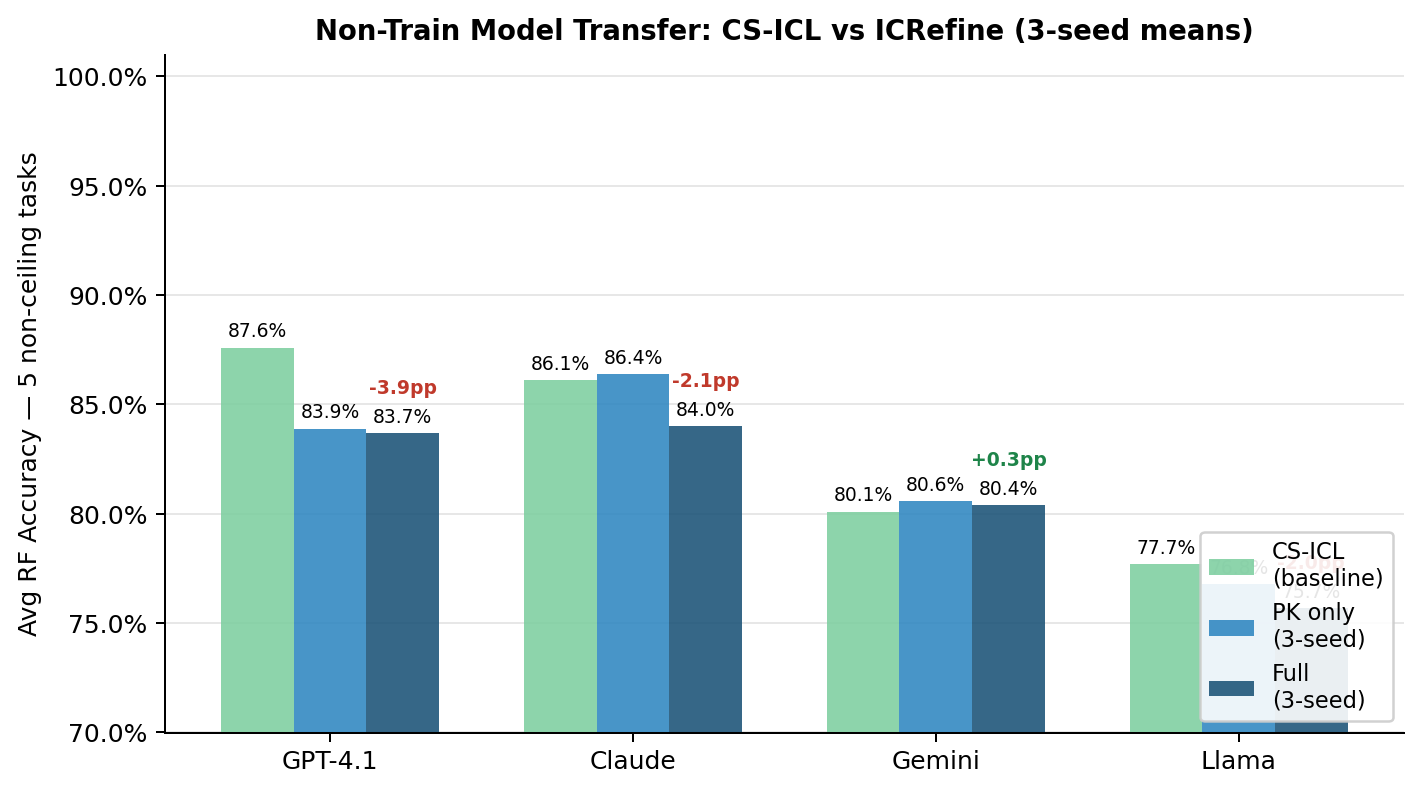
\includegraphics[width=0.85\linewidth]{fig2_nontrain_transfer.png}
  \caption{Non-train RF accuracy averaged over five non-ceiling tasks for each evaluation model
    under three conditions. PK-only transfers more consistently than the full cheatsheet across
    three of four model families, identifying Phase~2 case studies as the transfer bottleneck.}
  \label{fig:transfer}
\end{figure}

\paragraph{The transfer gap is task-structured, not model-structured.}
The locus of harm varies by task rather than by model family (Figure~\ref{fig:delta_cs}).
Causal\_judgement case studies reduce accuracy across all five models in the 3-seed mean:
$-4.2$\,pp (Claude), $-3.5$\,pp (Llama), $-2.3$\,pp (Gemini), $-0.8$\,pp (GPT-4.1),
and $+3.1$\,pp (train model, mini), indicating near-universally harmful case studies.
Geometric\_shapes case studies produce a more heterogeneous pattern in the 3-seed mean
($\Delta_\text{cs}$): mini $+1.3$\,pp, GPT-4.1 $-0.7$\,pp, Claude $-3.3$\,pp, Gemini $+2.0$\,pp,
Llama $-6.7$\,pp---consistent with models sharing the same SVG parsing failure modes
(mini, Gemini) benefiting while more capable spatial reasoners (Claude) are hurt.
This task-structured pattern---rather than a uniform model-size or model-family effect---
suggests that case study transferability depends on whether the failure mode the case study
encodes is shared across model families.
Formal, domain-structural failures (arc rotation classification, multi-subpath vertex counting)
are more likely to be shared; oracle-contaminated reasoning failures (a paraphrase of one
training item's gold chain-of-thought) mislead all models that encounter them.

\paragraph{A second training model yields results consistent with the task-structured pattern.}
To test whether the transfer gap reflects idiosyncrasies of gpt-4.1-mini, we re-ran the
full v3 pipeline with gemini-2.0-flash as the train model in all three roles
(scoring, rule-patching, case-study generation) on the same five tasks.
Table~\ref{tab:gemini_transfer} reports the results (3-seed means).
The task-structured pattern holds: CJ case study effects are small and mostly negative
(GPT $-0.4$\,pp, Llama $-0.8$\,pp, Gemini* $-2.3$\,pp; Claude $+1.5$\,pp is the sole
positive outlier), while GS case studies are broadly helpful for strong non-train
models---Claude gains $+11.3$\,pp and GPT-4.1 gains $+4.0$\,pp under Gemini training
(vs.\ $-3.3$\,pp and $-0.7$\,pp respectively under mini training), confirming that GS
case studies help models that lack mini's SVG parsing failure modes regardless of which
model generated the cheatsheet.
Concretely, the non-train $\Delta$ vs CS-ICL under Gemini training ($-3.7$, $-2.9$, $-3.5$\,pp
for GPT-4.1, Claude, Llama) are within 1\,pp of the mini-trained equivalents
($-3.4$, $-3.7$, $-2.6$\,pp).
All non-train models remain below CS-ICL under both training regimes.
This two-model comparison is consistent with the transfer gap being task-determined rather
than training-model-determined, though establishing this as a general property would require
testing additional training model conditions (e.g.\ Claude or Llama as train model).

% ── Table: Gemini-trained transfer ───────────────────────────
\begin{table}[t]
  \caption{Bidirectional transfer check: Gemini-2.0-flash as train model, full v3 pipeline,
    3-seed means (seeds 1--3). Non-train 5-task RF averages compared to mini-trained v3
    (3-seed mean) and CS-ICL. $\Delta_\text{cs}$ is full minus PK-only for CJ and GS.
    Gemini* denotes the train model.}
  \label{tab:gemini_transfer}
  \centering
  \smallskip
  \begin{tabular}{lrrrr}
    \toprule
    \textbf{Model} & \textbf{Gemini-trained} & \textbf{Mini-trained (v3)} & \textbf{CS-ICL} & $\boldsymbol{\Delta}$ \\
    \midrule
    mini         & 80.9\% & --- & --- & --- \\
    GPT-4.1      & 83.4\% & 83.7\% & 87.1\% & $-3.7$ \\
    Claude-3.7   & 84.8\% & 84.0\% & 87.7\% & $-2.9$ \\
    Llama-3.3    & 74.8\% & 75.7\% & 78.3\% & $-3.5$ \\
    Gemini-2.0*  & --- & 80.4\% & 81.4\% & --- \\
    \bottomrule
    \multicolumn{5}{l}{\footnotesize $\Delta$ = Gemini-trained full $-$ CS-ICL (non-train only). 3-seed means.} \\
    \multicolumn{5}{l}{\footnotesize CJ $\Delta_\text{cs}$: $-0.4$\,pp (GPT), $+1.5$\,pp (Claude), $-2.3$\,pp (Gemini*), $-0.8$\,pp (Llama).} \\
    \multicolumn{5}{l}{\footnotesize GS $\Delta_\text{cs}$: $+4.0$\,pp (GPT), $+11.3$\,pp (Claude), $+9.7$\,pp (Gemini*), $-5.3$\,pp (Llama).} \\
  \end{tabular}
\end{table}

% ── Figure 7 ─────────────────────────────────────────────────
\begin{figure}[t]
  \centering
  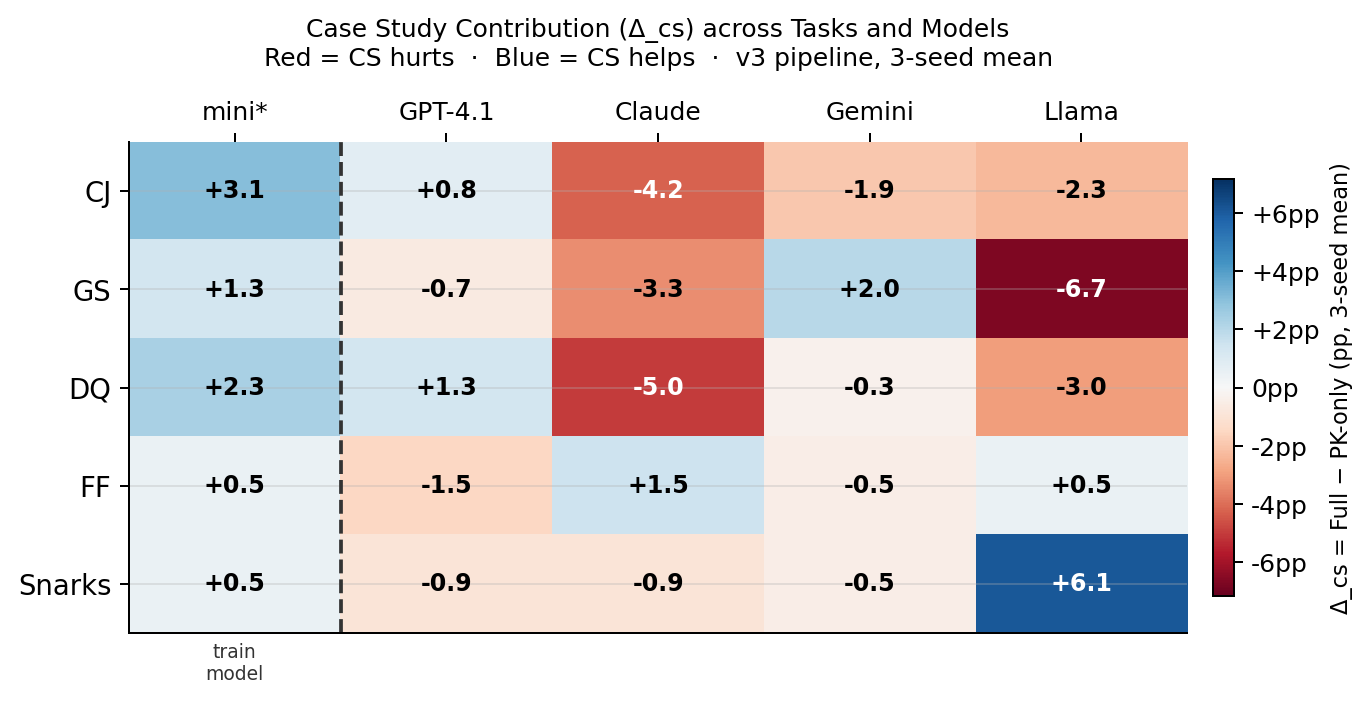
\includegraphics[width=0.85\linewidth]{fig7_delta_cs_heatmap.png}
  \caption{$\Delta_\text{cs}$ (full minus PK-only, in pp) heatmap over 5 tasks $\times$ 5 models,
    from v3 3-seed means. Blue cells: case studies help; red cells: case studies hurt.
    CJ shows uniformly negative case study contributions across all models (except mini, the
    train model), consistent with the failure modes characterised in Section~\ref{sec:oracle}. GS shows heterogeneous effects:
    positive for mini ($+1.3$\,pp) and Gemini ($+2.0$\,pp), negative for Claude ($-3.3$\,pp)
    and Llama ($-6.7$\,pp), consistent with model-specific SVG parsing capabilities.
    Dashed line separates the train model (mini) from non-train models.
    DQ (Claude $-5.0$\,pp) and Llama GS ($-6.7$\,pp) are the largest individual harms.
    FF is near-neutral across all models. Snarks is near-neutral except for Llama ($+6.1$\,pp),
    whose PK-only accuracy on Snarks is below ceiling ($83.1\%$), leaving room for case study benefit.}
  \label{fig:delta_cs}
\end{figure}

% ------------------------------------------------------------
\subsection{On-train performance}
\label{sec:overall}

On the training model (gpt-4.1-mini), Table~\ref{tab:phase_contribution} and
Figure~\ref{fig:phase_contribution} show a mixed picture across the five non-ceiling tasks.
\textbf{Formal\_fallacies} ($+2.0$\,pp vs.\ CS-ICL) and \textbf{geometric\_shapes}
($-5.0$\,pp vs.\ CS-ICL, 3-seed mean) show opposing Phase~2 effects: FF benefits from a
15-rule propositional logic taxonomy \emph{in its prior knowledge} (Phase~1 output; the four
Phase~2 case studies are near-duplicates, Section~\ref{sec:overfitting}) that encodes systematic
inference errors identified during iterative refinement, while GS Phase~2 case studies add $+5.0$\,pp over Phase~1
on the train model but the full pipeline still falls below the CS-ICL baseline
($74.0\%$ vs.\ $79.0\%$, train model 3-seed mean).
\textbf{Causal\_judgement} shows the largest Phase~2 penalty: $-5.7$\,pp relative to Phase~1,
and the full pipeline ($64.4\%$) falls $2.3$\,pp below CS-ICL ($66.7\%$).

Seven of eleven tasks saturate at or above 95\% after Phase~0 bootstrap alone (Bool, Nav, WOL,
LD3, Sports, FF, Snarks), leaving four tasks where iterative refinement produces non-trivial
cheatsheet content.
This saturation pattern suggests that iterative refinement may add value primarily for tasks
where the bootstrap PK leaves structured failure modes unaddressed---though this observation
is limited to the task distribution studied here and does not straightforwardly predict which
task families would benefit in a new application domain.

% ── Table 1 ──────────────────────────────────────────────────
\begin{table}[t]
  \caption{Phase contribution on the test set---gpt-4.1-mini, reasoning-first (RF) accuracy.
    \textit{Phase~0}: auto-bootstrap only. \textit{Phase~1 (PK)}: after iterative PK patching.
    \textit{Phase~2 (full)}: with case studies. $\Delta$\,P1$\!\to$P2 isolates the marginal
    case study contribution. Single-run results.}
  \label{tab:phase_contribution}
  \centering
  \smallskip
  \begin{tabular}{lrrrrc}
    \toprule
    \textbf{Task}
      & \textbf{CS-ICL}
      & \textbf{Phase 0}
      & \textbf{Phase 1}
      & \textbf{Phase 2}
      & $\boldsymbol{\Delta}$\,\textbf{P1$\!\to$\!P2} \\
    \midrule
    Bool   & 100.0\% & 100.0\% & 100.0\% & 100.0\% & $\phantom{+}0.0$ \\
    CJ     &  66.7\% &  73.6\% &  70.1\% &  64.4\% & $-5.7$ \\
    DU     &  95.0\% &  94.0\% &  91.0\% &  93.0\% & $+2.0$ \\
    DQ     &  91.0\% &  84.0\% &  87.0\% &  86.0\% & $-1.0$ \\
    FF     &  95.0\% &  96.0\% &  96.0\% &  97.0\% & $+1.0$ \\
    GS     &  79.0\% &  70.0\% &  71.0\% &  76.0\% & $\mathbf{+5.0}$ \\
    LD3    & 100.0\% & 100.0\% & 100.0\% & 100.0\% & $\phantom{+}0.0$ \\
    Nav    & 100.0\% & 100.0\% & 100.0\% & 100.0\% & $\phantom{+}0.0$ \\
    Snarks &  95.8\% &  95.8\% &  94.4\% &  95.8\% & $+1.4$ \\
    Sports &  98.0\% & 100.0\% &  99.0\% & 100.0\% & $+1.0$ \\
    WOL    & 100.0\% & 100.0\% & 100.0\% & 100.0\% & $\phantom{+}0.0$ \\
    \bottomrule
  \end{tabular}
\end{table}

% ── Figure 1 ─────────────────────────────────────────────────
\begin{figure}[t]
  \centering
  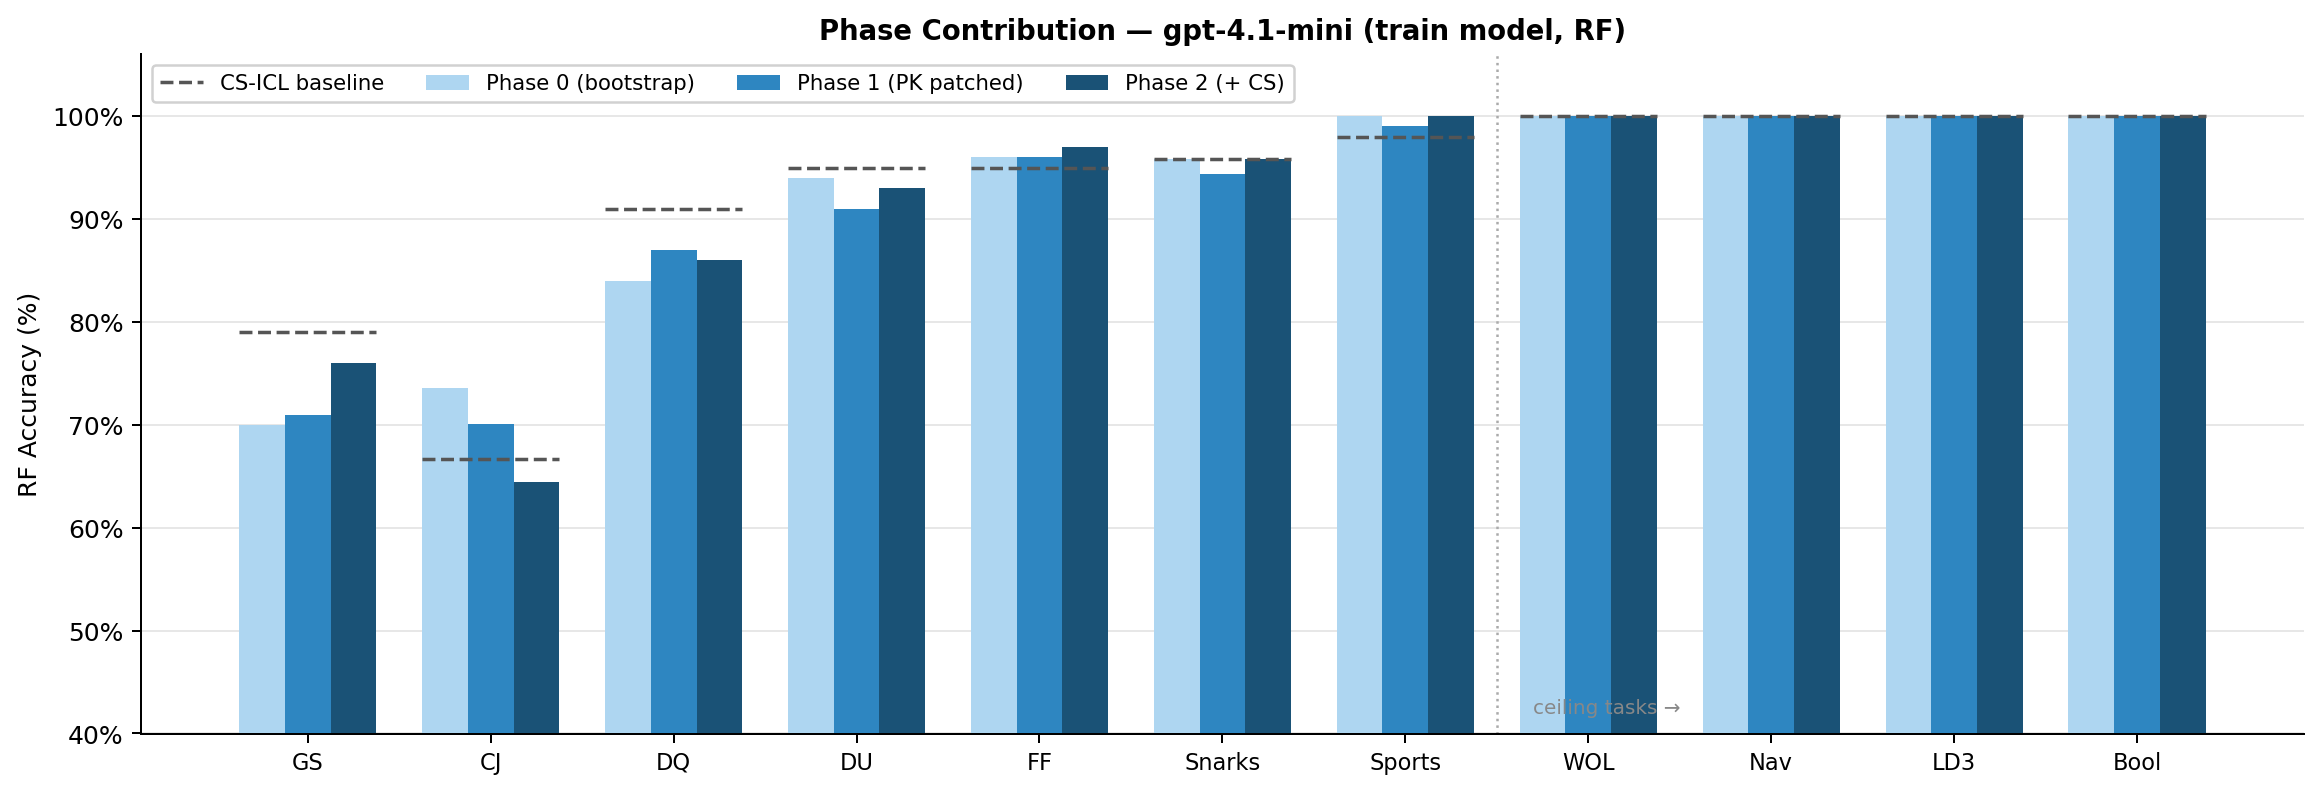
\includegraphics[width=\linewidth]{fig1_phase_contribution.png}
  \caption{RF test accuracy by pipeline phase for gpt-4.1-mini across all 11 BIG-Bench Hard
    tasks. Seven tasks reach $\geq$95\% after Phase~0 alone. Phase~2 case studies produce
    the largest task-level shift on geometric\_shapes ($+5.0$\,pp) and causal\_judgement
    ($-5.7$\,pp), illustrating both the potential and failure modes of partition-based case
    study generation.}
  \label{fig:phase_contribution}
\end{figure}

% ------------------------------------------------------------
\subsection{Mechanism 1: case study partition overfitting}
\label{sec:overfitting}

Phase~2 partitions the training set by error type and generates one case study per coherent
failure cluster.
This mechanism succeeds when failures concentrate in reproducible error classes, and fails when
they are dispersed or when the generated case studies are too specific to the train model's
exact error profile.

\paragraph{Geometric shapes: generalizable structural case studies.}
Listing~\ref{lst:gs_cs} shows the two GS case studies produced by v3.
Both ACTIVATE~IF conditions encode structural geometric rules: multi-subpath vertex counting
and arc rotation misclassification.
Unlike the CJ case study (which paraphrases a specific oracle trace), these rules are
intended to be structurally generalizable---the equal-radii-plus-nonzero-rotation condition
for arc/circle distinction applies to any model encountering SVG arc paths, not just gpt-4.1-mini.
One caveat: the \texttt{n\_vertices $\approx$ 7} predicate in CS1 is narrow;
its generalizability depends on whether GS test failures cluster around similar vertex counts,
which we have not directly verified.
This structural character explains why Phase~2 adds $+5.0$\,pp on the train model
(Table~\ref{tab:phase_contribution}).
In the 5-model, 3-seed transfer evaluation, GS case studies are near-neutral on average:
Gemini benefits most ($+2.0$\,pp) while Claude ($-3.3$\,pp) and Llama ($-6.7$\,pp) are
hurt---models that already parse SVG paths capably are confused by case studies optimised
for the train model's failure modes.
The full pipeline falls below the CS-ICL baseline ($74.0\%$ vs.\ $79.0\%$, 3-seed means)
because Phase~1 PK patching is limited on GS (Phase~1 achieves $72.7\%$, only $+2.7$\,pp
above Phase~0), and the Phase~2 gain for stronger models cannot offset the harm to weaker ones.

\begin{lstlisting}[caption={Phase-2 case studies generated for geometric\_shapes (v3). ACTIVATE
  IF conditions encode structural SVG parsing rules intended to generalise across model families
  (narrow predicates such as \texttt{n\_vertices}$\approx$7 limit scope):
  under Gemini training, these rules benefit GPT-4.1 ($+4.0$\,pp) and Gemini ($+5.0$\,pp).},
  label={lst:gs_cs}]
=== CS1: Correct vertex counting across multiple "M" subpaths ===
ACTIVATE IF:
  has_multi_subpath = true
  n_vertices ~= 7
  error = miscounted_vertices
WHY: Multiple M commands may form one connected polygon; endpoints shared
     across subpaths must be counted collectively, not per-subpath.

=== CS2: Arc paths misclassified as circles instead of ellipses ===
ACTIVATE IF:
  has_arc = true
  arc_radii_equal = true
  rotation_angle significantly non-zero
  model_predicts = circle
WHY: Equal radii alone do not classify an arc as a circle; the rotation
     angle must be near-zero for circle classification.
\end{lstlisting}

\paragraph{Formal fallacies: partition search fixation.}
Four case studies were generated for formal\_fallacies, but three (CS1, CS2, CS4) all address
illicit conversion of conditionals (premise: $A\!\Rightarrow\!B$; conclusion:
$B\!\Rightarrow\!A$); CS1 and CS4 are near-identical.
This redundancy reveals a limitation in the greedy partition search: Phase~2 encounters the
illicit-conversion failure type across multiple bins and generates a new case study each time
without detecting prior overlap.
Only CS3 (invalid inference from a disjunction premise) covers orthogonal ground.
Deduplication---checking new case study ACTIVATE~IF conditions against existing ones before
accepting---would resolve this and is a straightforward pipeline fix we leave for future work.

\paragraph{Causal judgement: oracle-contaminated specificity.}
Causal\_judgement has the most dispersed failure distribution: 35 training failures spanning
joint-AND causation, OR/redundant causes, prevention chains, norm violations, timing effects,
and intentionality judgements.
No single partition is large enough to yield a high fix-rate case study without regressing
others.
The single CJ case study that passed the acceptance gate (fix\_rate = 42\%) is shown in
Listing~\ref{lst:cj_cs}: a free-form narrative that closely paraphrases one specific training
item's oracle reasoning. \emph{Note: this seed~1 case study is atypical---seeds~2 and~3 generate
structurally formatted ACTIVATE-IF case studies rather than free-form narratives---yet both
also reduce accuracy (Appendix~\ref{sec:cj_casestudies}), implicating failure-distribution
heterogeneity as a co-cause independent of oracle format.}
This oracle-derived specificity is a plausible primary contributor to the $-5.7$\,pp Phase~2
penalty: the case study encodes reasoning steps for one idiosyncratic joint-AND scenario,
misleading the model on unrelated causal question types.
An alternative co-explanation is CJ's inherently heterogeneous failure distribution---35 training
failures spanning joint-AND causation, OR/redundant causes, prevention chains, norm violations,
timing effects, and intentionality judgements---which makes any single case study prone to
overfitting regardless of oracle access.
The oracle ablation in Section~\ref{sec:oracle} tests whether removing oracle access reduces
the Phase~2 penalty; the residual gap after oracle removal provides evidence on which factor
dominates.
The cross-seed case study inventory (Appendix~\ref{sec:cj_casestudies}) further characterises
this: seeds~2 and 3 produce case studies that are \emph{not} oracle-contaminated in form,
yet still reduce accuracy, implicating failure-distribution heterogeneity as a co-cause.
Critically, this harm is not limited to the train model---the 5-model 3-seed evaluation shows
Phase~2 reducing accuracy for Claude ($-4.2$\,pp), Gemini ($-1.9$\,pp), and Llama ($-2.3$\,pp);
GPT-4.1 shows a marginal $+0.8$\,pp gain (Section~\ref{sec:oracle} and Figure~\ref{fig:delta_cs}).

\begin{lstlisting}[caption={The single Phase-2 case study generated for causal\_judgement (v3).
  Free-form prose paraphrasing one training item's oracle reasoning, encoding the train
  model's idiosyncratic treatment of joint-AND causation.},
  label={lst:cj_cs}]
=== Joint causes (logical AND): garden fertilizers ===
Scenario: Two gardeners independently apply fertilizers; plants dry out
  only if BOTH fertilizers are applied simultaneously.
Verdict: NO (neither gardener alone caused it)
Apply when: outcome requires simultaneous co-occurrence of conditions
  (logical AND)---neither party alone is causally responsible.
\end{lstlisting}

% ------------------------------------------------------------
\subsection{Mechanism 2: oracle contamination}
\label{sec:oracle}

Phase~2 injects the gold chain-of-thought (\texttt{item["reason"]}) into failure-analysis
prompts during case study generation.
Experiment E3 tests the causal role of oracle access by re-running the CJ pipeline with
both Phase~1 and Phase~2 oracle contexts disabled (\texttt{--no-oracle}).

\paragraph{Oracle-free Phase~2 generates more transferable case studies.}
Unlike an earlier CoT-mode ablation that disabled only the Phase~2 oracle and produced zero
case studies, the RF-mode E3 condition (\texttt{--no-oracle} on both phases) still generates
Phase~2 case studies---the model synthesises correction rules from prediction failures alone,
without gold reasoning.
These oracle-free case studies are directionally helpful: Table~\ref{tab:e3_oracle} and
Figure~\ref{fig:oracle_gradient} show that all five models improve under E3, using 3-seed
means for both conditions.
Improvements range from $+1.9$\,pp (mini, Gemini) to $+3.8$\,pp (Llama), with GPT-4.1 gaining
$+3.1$\,pp and Claude $+3.5$\,pp.
The consistent direction across all models and across all three pipeline seeds
(see Figure~\ref{fig:variance}) is consistent with oracle injection being a
\emph{contributing factor} in the CJ case study's harm---oracle-free case studies avoid the
most acute form of this failure mode.
Effect sizes are moderate (all $\leq 4$\,pp); the benefit of removing oracle access is real
but not large in absolute terms.
E3 CJ does \emph{not} fully recover CS-ICL performance: the non-train E3 average
($68.5\%$) remains $3.9$\,pp below the CS-ICL CJ average ($72.4\%$)---comparable in size to
the oracle-removal effect itself ($+1.9$--$+3.8$\,pp).
This residual gap is consistent with heterogeneous failure distribution being a co-contributing
cause: even oracle-free case studies may overfit when CJ failures span six or more structurally
distinct subtypes.
Oracle contamination removal narrows but does not close the gap; CJ case study generation
remains difficult regardless of oracle access.

% ── Table E3 ─────────────────────────────────────────────────
\begin{table}[t]
  \caption{E3 oracle ablation on causal\_judgement (RF, 5 models). E3: both Phase~1 and Phase~2
    oracle disabled (\texttt{--no-oracle}); Phase~2 generates case studies without gold
    chain-of-thought. v3 full: standard oracle-enabled pipeline. $\Delta$\,=\,E3 full\,$-$\,v3 full.
    \textbf{Both columns are 3-seed means} (E3 and v3 each averaged over 3 independent pipeline
    runs); improvements range from $+1.9$ to $+3.8$\,pp.
    The train model (mini*, $+1.9$\,pp) and Gemini ($+1.9$\,pp) improvements approach the
    2--4\,pp noise floor; non-train improvements for GPT-4.1 ($+3.1$\,pp), Claude ($+3.5$\,pp),
    and Llama ($+3.8$\,pp) are more robustly above it.
    * denotes the training model.}
  \label{tab:e3_oracle}
  \centering
  \smallskip
  \begin{tabular}{lrrr}
    \toprule
    \textbf{Model} & \textbf{E3 (no oracle)} & \textbf{v3 full} & $\boldsymbol{\Delta}$ \\
    \midrule
    gpt-4.1-mini*  & 69.7\% & 67.8\% & $+1.9$ \\
    gpt-4.1        & 70.5\% & 67.4\% & $+3.1$ \\
    claude-3.7     & 69.0\% & 65.5\% & $+3.5$ \\
    gemini-2.0     & 65.9\% & 64.0\% & $+1.9$ \\
    llama-3.3      & 68.6\% & 64.8\% & $+3.8$ \\
    \bottomrule
  \end{tabular}
\end{table}

% ── Figure 8 ─────────────────────────────────────────────────
\begin{figure}[t]
  \centering
  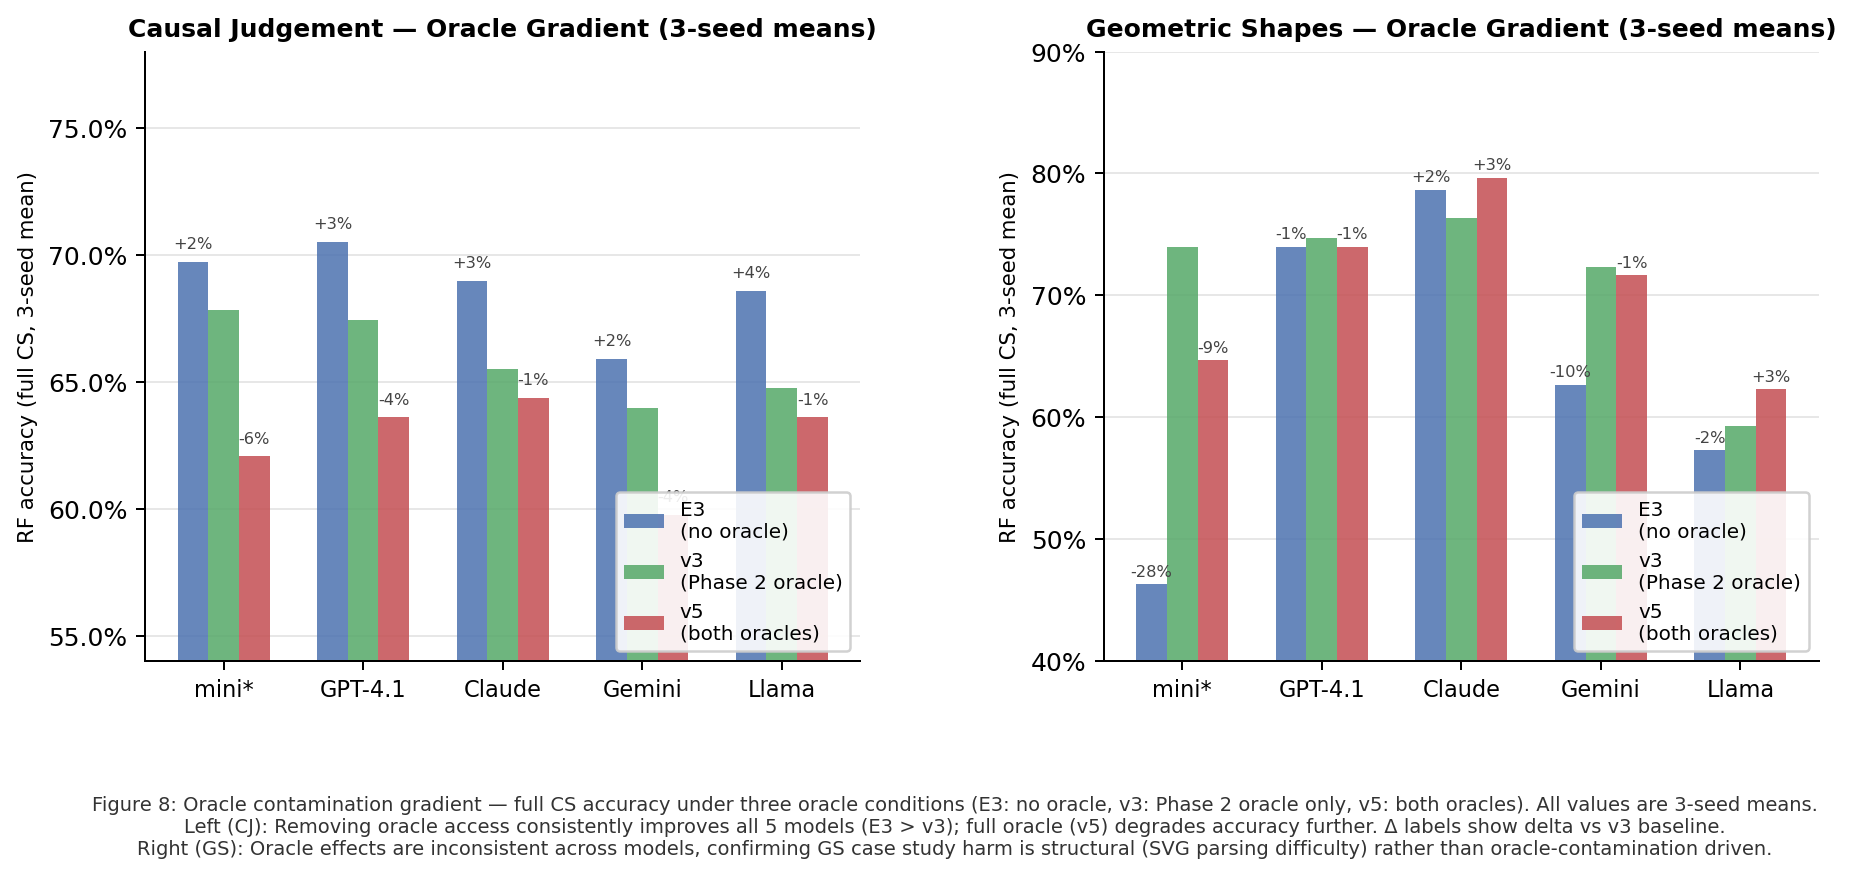
\includegraphics[width=0.85\linewidth]{fig8_oracle_gradient.png}
  \caption{Oracle contamination gradient on causal\_judgement (left, full CS accuracy) and
    geometric\_shapes (right, full CS accuracy) across three oracle conditions: E3 no-oracle,
    v3 standard (Phase~2 oracle only), and v5 full-oracle (both Phase~1 and Phase~2 oracle
    enabled). All values are 3-seed means. On CJ, removing oracle access consistently
    improves transfer: E3 $>$ v3 for 4 of 5 models; full oracle (v5) degrades accuracy further
    for GPT-4.1, Gemini, and Llama. On GS, oracle effects are less consistent, reflecting
    that GS case study harm is structural (SVG parsing) rather than oracle-contamination driven.}
  \label{fig:oracle_gradient}
\end{figure}

The oracle dilemma has a design implication: oracle injection may assist Phase~2 case study
generation on tasks with heterogeneous failure distributions, but simultaneously risks
encoding reasoning specificity that does not transfer.
The E3 result suggests that for CJ specifically, oracle-free generation already produces
adequate case study material---the gold chain-of-thought is not required to identify
generalizable correction rules, and providing it causes overfit to specific oracle reasoning
styles.
The contrast with GS (where oracle-assisted case studies encode formally generalizable
geometric rules) indicates that the appropriate use of oracle context depends on whether
the failure mode admits a principled, item-independent correction rule.
Notably, seeds~2 and 3 of the v3 pipeline generate structurally general, non-oracle-contaminated
case studies for CJ (Appendix~\ref{sec:cj_casestudies})---yet these seeds still reduce
transfer accuracy below CS-ICL.
This confirms that failure-distribution heterogeneity is an independent contributing factor
beyond oracle contamination: the CJ failure space (35 instances spanning $\geq 6$
structurally distinct causal sub-types) is simply too diverse for case study-based
correction to generalise reliably, regardless of oracle access.
Figure~\ref{fig:gs_oracle_variance} confirms this interpretation: the within-condition
seed-to-seed variance on GS is high and the oracle ordering is non-monotone, whereas
on CJ the E3 improvement is consistent across all seeds (Figure~\ref{fig:variance}).

% ── Figure 9 ─────────────────────────────────────────────────
\begin{figure}[t]
  \centering
  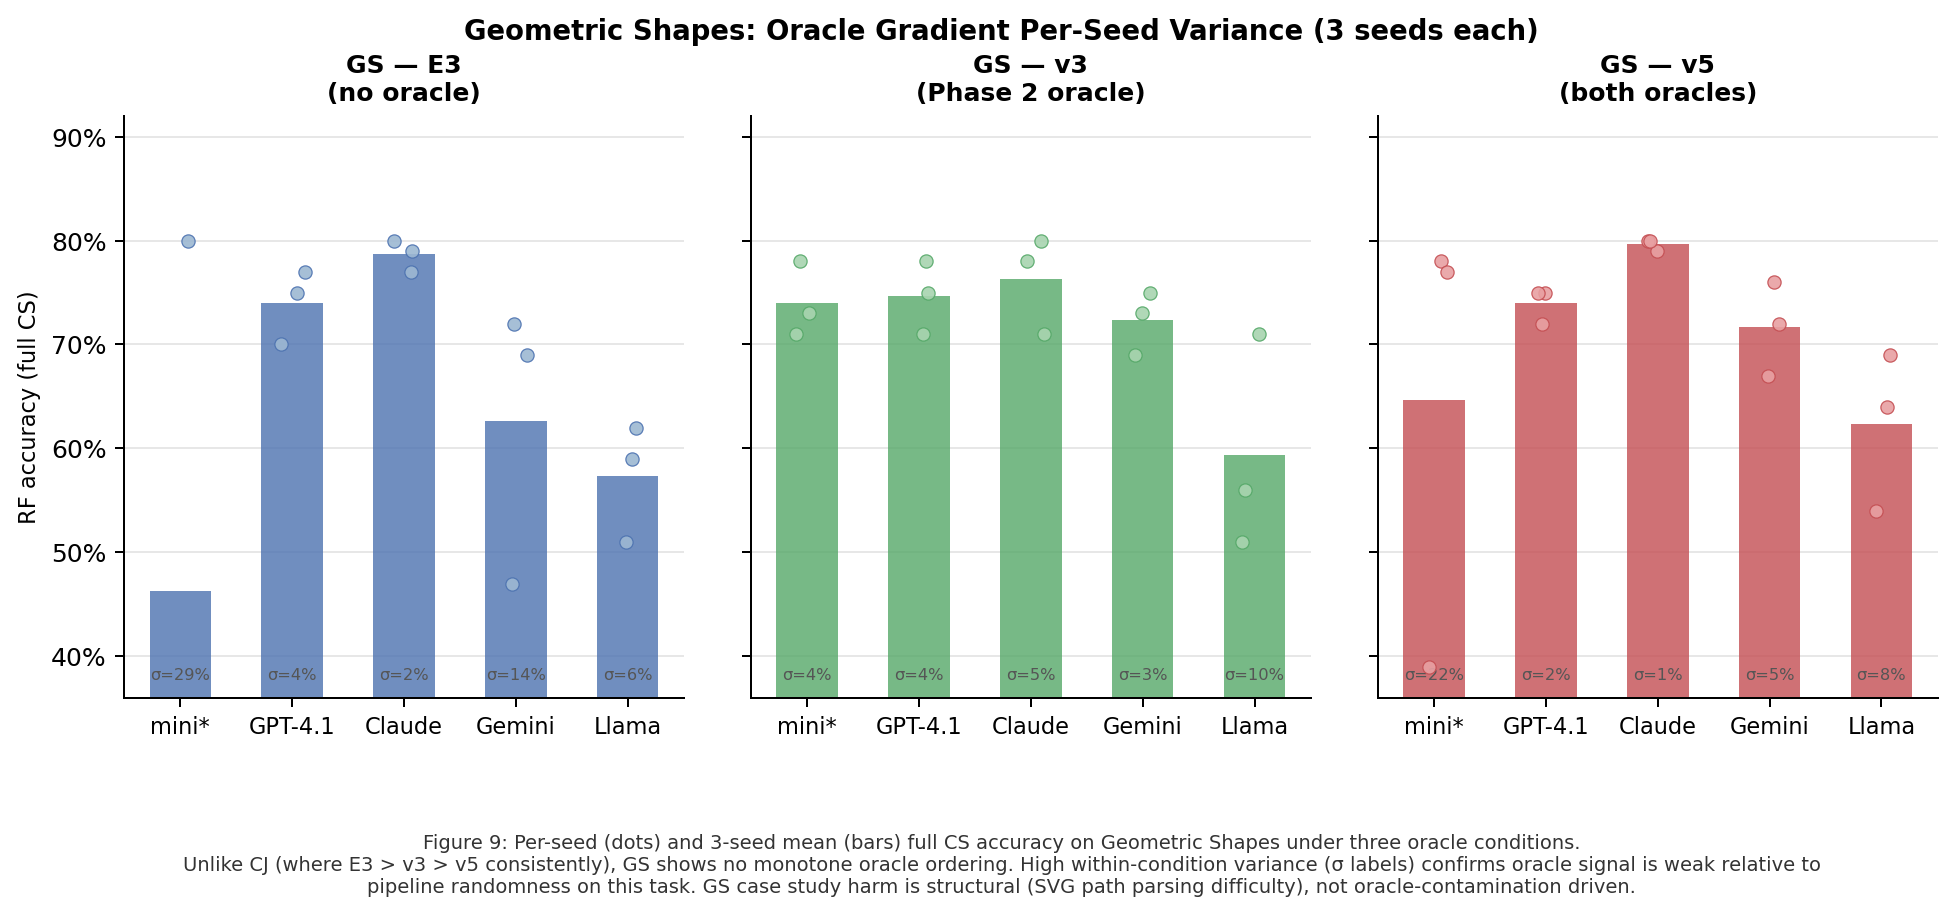
\includegraphics[width=\linewidth]{fig9_gs_oracle_variance.png}
  \caption{Per-seed (dots) and 3-seed mean (bars) full CS accuracy on geometric\_shapes
    under E3 (no oracle), v3 (Phase~2 oracle), and v5 (both oracles).
    Unlike causal\_judgement---where E3 $>$ v3 holds for all seeds and all models---GS shows
    no consistent oracle ordering.
    Within-condition $\sigma$ values (bottom labels) are 3--10\,pp, comparable to the
    cross-condition differences, confirming that oracle injection provides no reliable signal
    on this task.
    GS case study harm is structural (SVG path parsing difficulty) rather than
    oracle-contamination driven.}
  \label{fig:gs_oracle_variance}
\end{figure}

% ------------------------------------------------------------
\subsection{Mechanism 3: bootstrap convergence and sequential patching limits}
\label{sec:phases}

Phase~1 applies sequential PK patching: each iteration generates a single candidate revision,
accepts or rejects it on accuracy delta against the current PK, and moves on.
When the bootstrap PK already satisfies the acceptance gate---because the LLM generates a
sufficiently accurate initial cheatsheet from 75 training examples---Phase~1 applies zero
patches.
We observe this on five ceiling tasks (Bool, LD3, Nav, WOL, FF) where Phase~0 and Phase~1
accuracy are equal to within evaluation noise ($\geq$96\% throughout), and on geometric\_shapes
where Phase~1 adds only $+1.0$\,pp above Phase~0.
On CJ and DQ, Phase~1 does apply revisions but the gains are small: DQ improves
$+3.0$\,pp from Phase~0 to Phase~1 (both single-run).
CJ shows the opposite effect: the 3-seed Phase~1 mean ($64.8\%$) falls $8.8$\,pp below
the single-run Phase~0 bootstrap ($73.6\%$).
To avoid conflating single-run and 3-seed estimates, we note that all three individual
Phase~1 seeds also fall below this single-run baseline ($63.2\%$, $66.7\%$, $64.4\%$),
confirming a genuine Phase~1 failure rather than a comparison artefact.
This is consistent with the oracle contamination finding in Section~\ref{sec:oracle}:
Phase~1 failure signals on CJ are oracle-contaminated, so iterative patching reinforces
idiosyncratic reasoning patterns rather than improving generalizable rules.

Figure~\ref{fig:phase_contribution} shows the phase breakdown.
The $\Delta$\,P1$\!\to$\!P2 column confirms that Phase~2 is the variance-introducing step:
it produces the largest positive contribution ($+5.0$\,pp on GS) and the largest negative
contribution ($-5.7$\,pp on CJ).

% ------------------------------------------------------------
\subsection{Intervention: evolutionary algorithm Phase~1}
\label{sec:ea}

To address bootstrap convergence, we introduce an \textbf{Evolutionary Algorithm (EA) Phase~1}
that replaces single-candidate patching with population-based search: at each generation,
three candidate PK rewrites are scored in parallel on a held-out validation set (20\% of
training), and the top two survivors are recombined into the next generation via crossover.

Table~\ref{tab:ea} compares EA vs.\ standard Phase~1 on RF test accuracy using the PK-only
cheatsheet (prior knowledge without case studies), which isolates Phase~1 quality from
Phase~2 effects.

\paragraph{EA addresses the GS bootstrap convergence case.}
Standard Phase~1 applies zero patches to GS, yielding a PK-only test accuracy of $72.7\%$
averaged over three seeds.
EA Phase~1 applies three patches, raising PK-only test accuracy to $78.7\%$ ($+6.0$\,pp,
3-seed mean), and produces a cheatsheet with \emph{zero} case studies---the evolutionary
search finds a PK that encodes vertex-counting and arc-classification corrections directly in
the prior knowledge.
This improvement in PK quality substantially reduces the gap to the CS-ICL baseline:
EA PK alone ($78.7\%$) is approximately at the CS-ICL reference ($79.0\%$) on the train model.
The EA advantage is consistent across all three seeds and across all five evaluation models
(Figure~\ref{fig:variance}), confirming that the GS improvement is a genuine pipeline effect
rather than a single-run artifact; EA also exhibits lower seed-to-seed variance than
standard Phase~1 (Llama $\sigma=4.7\%$ vs.\ $10.4\%$).
Notably, EA's improved PK \emph{eliminates} Phase~2 case studies entirely for GS: the
acceptance gate rejects all candidates (zero case studies generated vs.\ two in standard Phase~1),
meaning the EA pipeline is purely PK-based for this task.
The evolutionary search encodes GS corrections---vertex counting and arc classification---directly
in prior knowledge at sufficient quality that no case study is needed.

\paragraph{Results on other tasks.}
PK character limit and Phase~2 case study count ablations are reported in
Appendix~\ref{sec:size_appendix}.
Across 3-seed means, EA improves CJ PK accuracy by $+5.4$\,pp ($70.1\%$ vs.\ $64.8\%$
standard), despite applying zero patches in seed~1.
However, the EA full-pipeline accuracy on CJ is \emph{lower} than standard
($64.4\%$ vs.\ $67.8\%$), because the four case studies EA generates on CJ
are oracle-contaminated and hurt evaluation-time accuracy---reinforcing the Phase~2
oracle contamination finding from Section~\ref{sec:oracle}.
Unlike v3 seed~1's free-form narrative paraphrase, EA's CJ case studies are structurally
formatted (ACTIVATE-IF) but remain oracle-derived in content, encoding joint-AND
causation patterns drawn from specific training examples.
The EA+no-oracle combined pipeline (Section~\ref{sec:combined}) pairs EA's improved CJ prior
knowledge with oracle-free Phase~2 case studies, thereby applying both interventions
simultaneously for CJ; the CJ slice of EA+no-oracle therefore uses EA Phase~1 PK, not standard Phase~1.
On Snarks and DQ, EA is within noise: $-0.9$\,pp and $0.0$\,pp respectively.
We do not claim EA as a general improvement over sequential patching beyond the GS case.

% ── Table 5 ──────────────────────────────────────────────────
\begin{table}[t]
  \caption{EA Phase~1 vs.\ standard Phase~1---RF test accuracy on gpt-4.1-mini.
    \textit{PK only}: cheatsheet without case studies evaluated on test set.
    \textit{Full}: complete pipeline (PK + Phase~2 case studies).
    EA: population size 3, 2 survivors, 12\,K-char PK budget, 20\% hold-out.
    Std CS / EA CS: number of Phase~2 case studies retained in each condition.
    \textbf{All PK columns are 3-seed means} (seeds 1--3 for both conditions);
    CS counts and patch counts are from seed~1.}
  \label{tab:ea}
  \centering
  \smallskip
  \begin{tabular}{lrrrrrr}
    \toprule
    \textbf{Task}
      & \textbf{Std PK}
      & \textbf{Std CS}
      & \textbf{EA PK}
      & \textbf{EA CS}
      & \textbf{EA patches}
      & $\boldsymbol{\Delta}$\,\textbf{PK} \\
    \midrule
    CJ     & 64.8\% & 1 & \textbf{70.1\%} & 4 & 0 & $+5.4$ \\
    GS     & 72.7\% & 2 & \textbf{78.7\%} & 0 & 3 & $+6.0$ \\
    Snarks & 96.7\% & 2 & 95.8\%          & 1 & 0 & $-0.9$ \\
    DQ     & 84.7\% & 0 & 84.7\%          & 3 & 1 & $\phantom{+}0.0$ \\
    \bottomrule
  \end{tabular}
\end{table}

% ── Figure 5 ─────────────────────────────────────────────────
\begin{figure}[t]
  \centering
  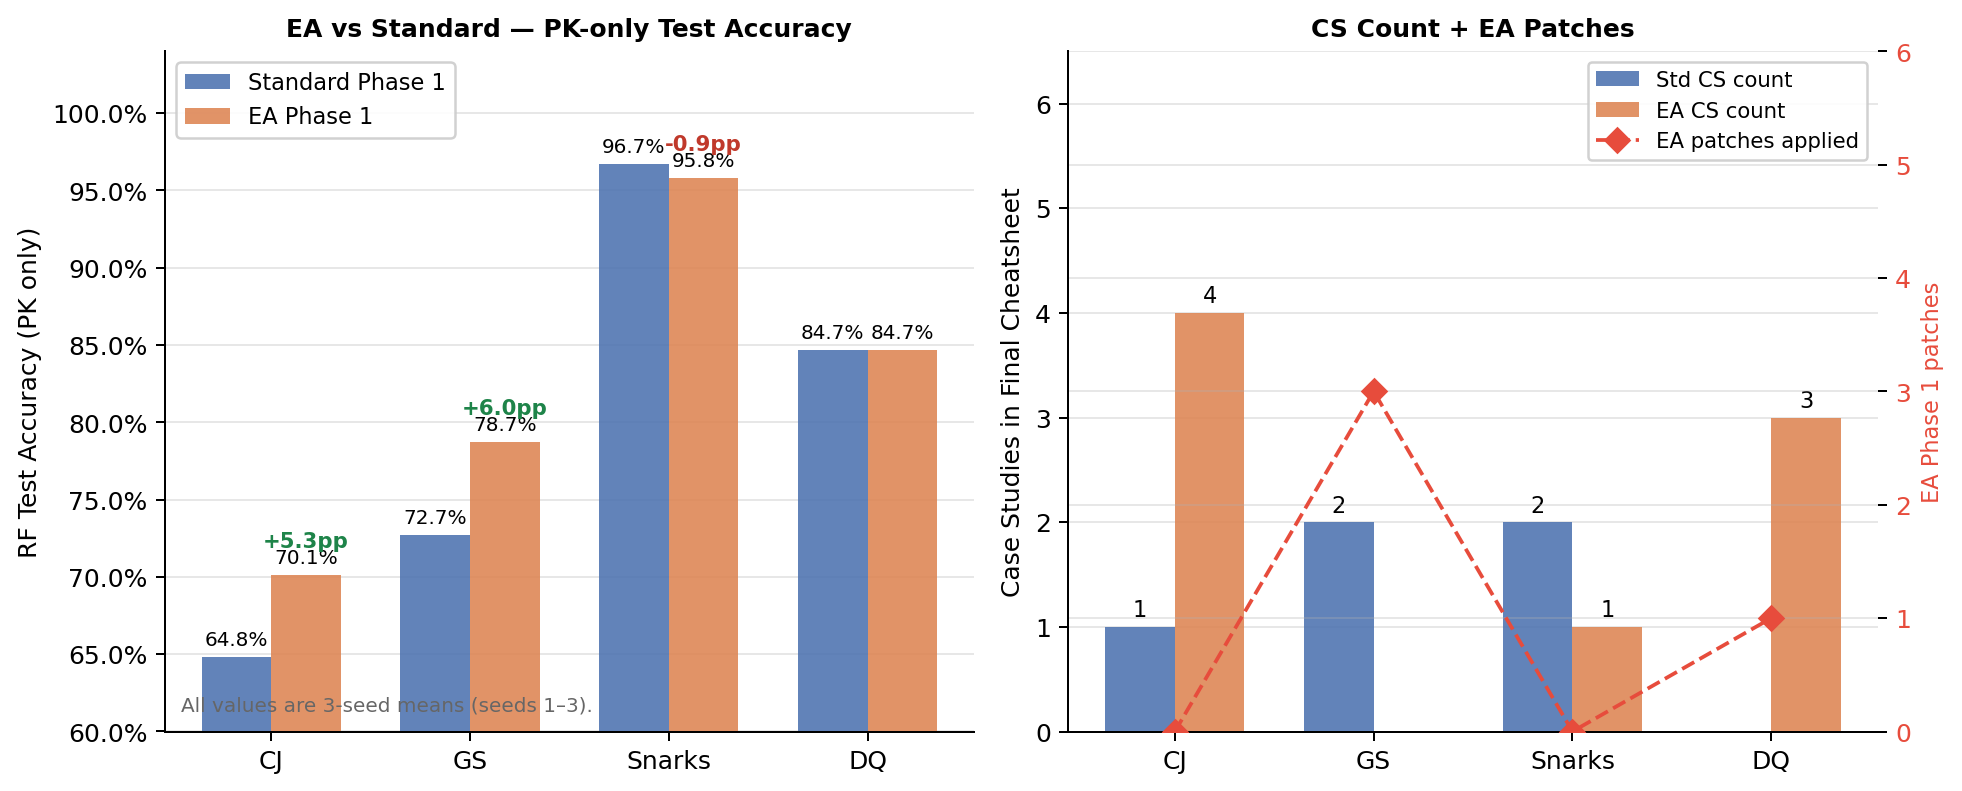
\includegraphics[width=0.85\linewidth]{fig5_ea_vs_standard.png}
  \caption{EA Phase~1 vs.\ standard Phase~1---RF test PK-only accuracy for four non-ceiling
    tasks (all 3-seed means, train model). GS is the primary beneficiary ($+6.0$\,pp),
    eliminating Phase~2 case studies entirely. CJ shows a consistent $+5.4$\,pp PK
    improvement; Snarks and DQ are within noise ($-0.9$\,pp and $0.0$\,pp respectively).}
  \label{fig:ea}
\end{figure}

% ------------------------------------------------------------
\subsection{Combined interventions: does the best-available pipeline beat CS-ICL?}
\label{sec:combined}

We address the central diagnostic question with two comparisons.
First, \textbf{EA+no-oracle}: a single coherent pipeline applying EA Phase~1 and
oracle-free Phase~2 across all five tasks uniformly (3-seed means).
Second, \textbf{best-combo}: a per-task oracle that selects the optimal intervention
independently per task (EA PK-only for GS; oracle-free E3 for CJ; v3 full for FF, DQ, Snarks).
Best-combo is not deployable---it requires knowing which intervention wins per task without
evaluation labels---and is best understood as an informal upper bound rather than a
rigorous one: selecting the best of 3 candidate interventions across 5 tasks introduces
multiple-comparisons inflation that is non-trivial relative to the 2--4\,pp noise floor.

Table~\ref{tab:combined} reports both.
EA+no-oracle remains below CS-ICL for all four model families: GPT-4.1 ($-3.3$\,pp),
Claude ($-2.4$\,pp), Gemini ($-0.6$\,pp), and Llama ($-3.6$\,pp).
Bootstrap CIs (95\%, task-resampling) exclude zero for GPT-4.1 and Claude; Gemini and Llama
CIs cross zero.
Best-combo adds $0.1$--$2.9$\,pp over EA+no-oracle depending on the model, confirming
that the per-task oracle margin is small.
All four families improve over the uncorrected v3 full pipeline under both comparisons.

Three cautions apply.
First, the CJ intervention (E3) improves \emph{over v3} for all models but does not reach
CS-ICL on CJ specifically: E3 CJ non-train average is $68.5\%$ vs.\ CS-ICL CJ $72.4\%$---
oracle contamination removal narrows the gap but does not close it.
Second, EA+no-oracle does not reach CS-ICL parity for GPT-4.1 ($-3.3$\,pp) or Llama ($-3.6$\,pp);
for these model families the residual transfer gap---driven predominantly by CJ and a
Llama-specific GS regression---is not addressable by the interventions studied here.
Third, all averages are backed by 3-seed means throughout; measurement noise is not the
primary uncertainty.

% ── Table 6 ──────────────────────────────────────────────────
\begin{table}[t]
  \caption{EA+no-oracle and best-combo vs.\ CS-ICL---non-train 5-task RF average (3-seed means).
    EA+no-oracle is a single coherent pipeline (EA Phase~1, oracle-free Phase~2) applied
    uniformly across all five tasks.
    Best-combo applies the best available intervention per task (EA PK-only for GS;
    E3 full for CJ; v3 full for FF/DQ/Snarks).
    $\Delta$\,=\,EA+no-oracle\,$-$\,CS-ICL; 95\% CI bootstraps over 5 tasks.
    $^{*}$\,CI excludes zero. $\dagger$\,Best-combo is a per-task oracle, not a deployable pipeline.
    \textbf{CS-ICL column is the same 3-seed mean as Table~\ref{tab:transfer}.}}
  \label{tab:combined}
  \centering
  \smallskip
  \begin{tabular}{lrrrrl}
    \toprule
    \textbf{Model} & \textbf{CS-ICL} & \textbf{EA+no-oracle} & $\boldsymbol{\Delta}$ & \textbf{Best-combo$^\dagger$} & \textbf{95\% CI} \\
    \midrule
    GPT-4.1    & 87.1\% & 83.8\% & $-3.3$ & 84.9\% & $[-6.3,\,-1.6]^{*}$ \\
    Claude-3.7 & 87.7\% & 85.3\% & $-2.4$ & 85.4\% & $[-5.4,\,-0.0]^{*}$ \\
    Gemini-2.0 & 81.4\% & 80.8\% & $-0.6$ & 81.2\% & $[-2.7,\,+1.6]$ \\
    Llama-3.3  & 78.3\% & 74.7\% & $-3.6$ & 77.6\% & $[-6.4,\,+0.8]$ \\
    \bottomrule
  \end{tabular}
\end{table}

% ------------------------------------------------------------
\subsection{Seed variance analysis}
\label{sec:variance}

API evaluations via OpenRouter show backend-routing non-determinism even at temperature zero,
producing 2--4\,pp across-run variance on difficult tasks.
To assess whether our key findings are robust to this noise, we ran the v3, E3, and EA
pipelines three times each from independent API calls (seeds 1--3) and report 3-seed means
throughout Sections~\ref{sec:transfer}--\ref{sec:ea}.

Figure~\ref{fig:variance} shows per-seed results for the two most informative comparisons.

\paragraph{GS: EA improvement is consistent and exhibits lower variance.}
The EA Phase~1 PK-only advantage over v3 ($+6.0$\,pp train-model mean) holds in all three
seeds for 4 of 5 models.
More strikingly, the EA cheatsheet is substantially \emph{more stable}: Llama's GS seed-to-seed
standard deviation drops from $\sigma=10.4$\,pp (v3) to $\sigma=4.7$\,pp (EA).
The high v3 Llama variance ($51\%$, $56\%$, $71\%$ across seeds) indicates that v3's GS
cheatsheet encodes rules that Llama applies inconsistently, while EA's cheatsheet is
structurally cleaner.

\paragraph{CJ: oracle-free improvement holds for all models across all seeds.}
The E3 advantage over v3 is positive for every model in every seed.
The 3-seed means show uniform improvement across all five model families ($+1.9$ to $+3.8$\,pp),
making this the strongest cross-seed result in our evaluation.
The single-run E3 numbers for GPT-4.1 ($+8.1$\,pp) and Llama ($+8.0$\,pp) were inflated
because the corresponding v3 seeds happened to be weak; the 3-seed comparison reveals a
more modest but consistent benefit.

% ── Figure 6 ─────────────────────────────────────────────────
\begin{figure}[t]
  \centering
  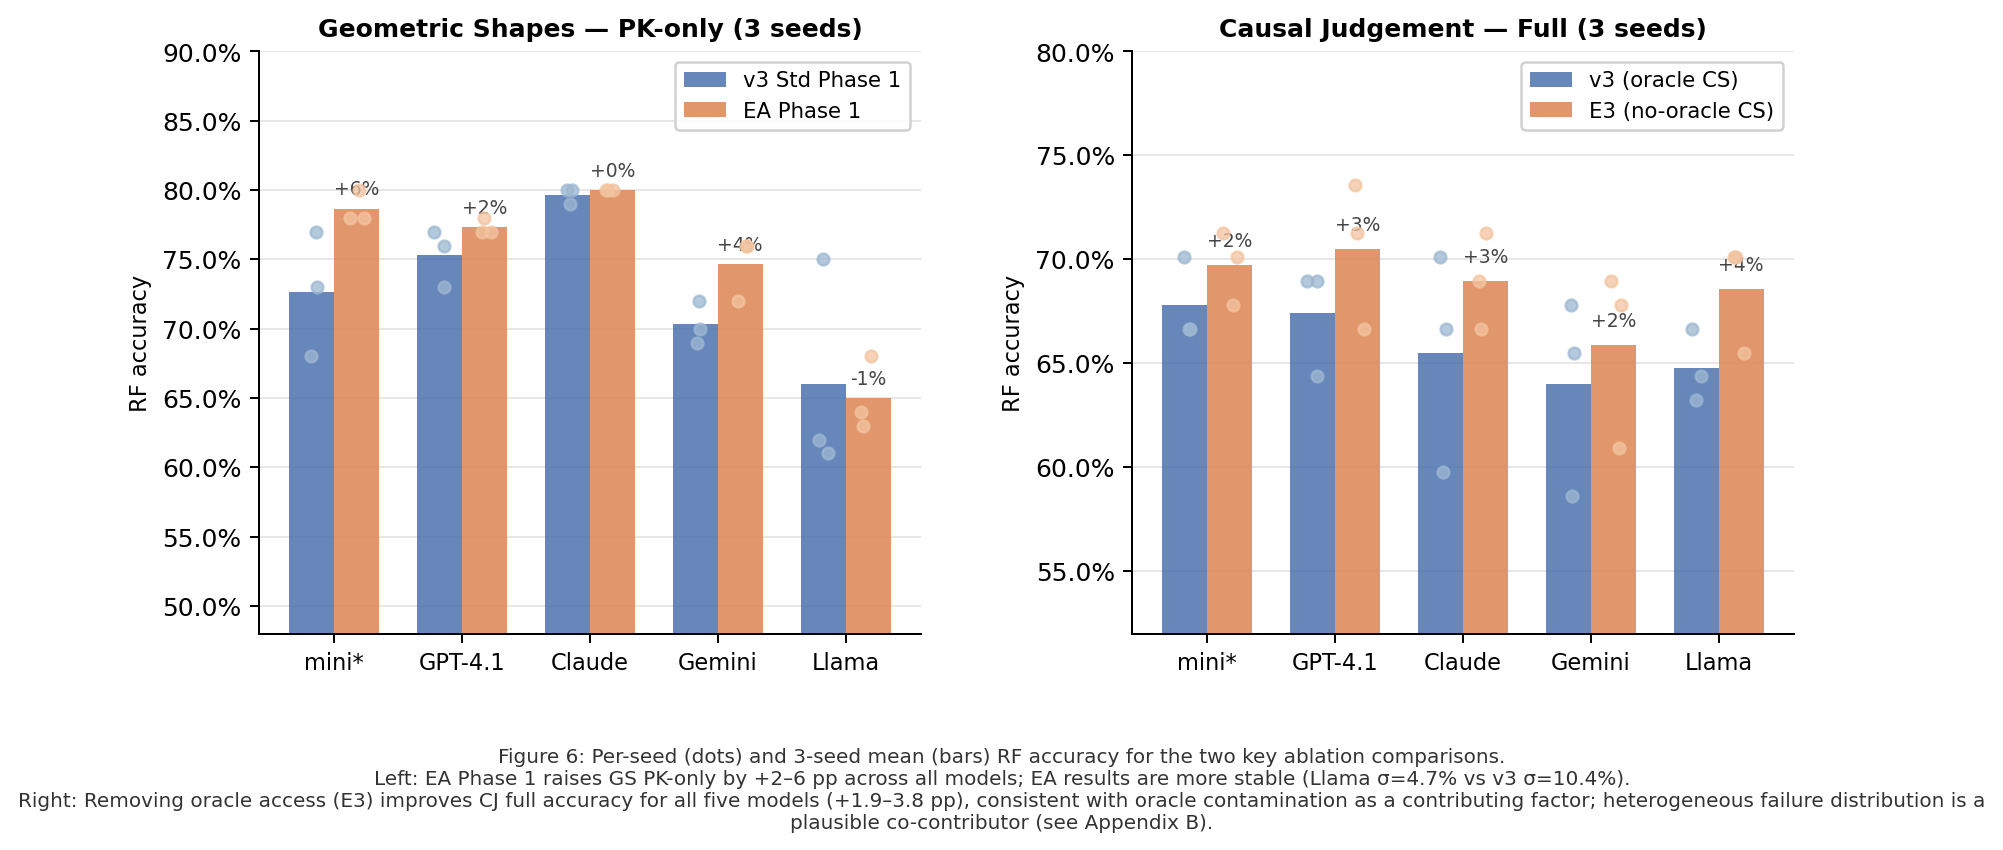
\includegraphics[width=\linewidth]{fig6_variance_analysis.png}
  \caption{Per-seed (dots) and 3-seed mean (bars) RF accuracy for two key ablation pairs.
    \textit{Left}: EA Phase~1 raises GS PK-only accuracy by $+2$ to $+6$\,pp across models;
    EA seed-to-seed variance is substantially lower (Llama $\sigma=4.7\%$ vs.\ $10.4\%$).
    \textit{Right}: Removing oracle access (E3) improves CJ full accuracy for all five
    models by $+1.9$ to $+3.8$\,pp, consistent with oracle contamination as a contributing
    factor in v3 CJ case study harm; heterogeneous failure distribution is a plausible
    co-contributor (Section~\ref{sec:oracle}).
    Percentage labels show $\Delta$ (comparison minus v3 baseline).}
  \label{fig:variance}
\end{figure}

% ------------------------------------------------------------
\subsection{Limitations}
\label{sec:limits}

The bidirectional transfer check (Section~\ref{sec:transfer}, Table~\ref{tab:gemini_transfer})
is based on two training models; the task-determined framing would be strengthened by a third.
BIG-Bench Hard test sets contain 87--250 examples per task, meaning a 1\,pp difference
corresponds to 1--2 examples; differences below 3\,pp should be interpreted cautiously.

\textbf{CS-ICL baseline.}
CS-ICL is now re-scored over three independent seeds with the same RF prompting as all
\textsc{ICRefine} conditions, resolving the earlier single-run asymmetry.
Differences between the 3-seed CS-ICL means and the original single-run values are $\leq 1.3$\,pp,
confirming that CS-ICL evaluation is stable across seeds.
CS-ICL is generated by gpt-4.1 (not gpt-4.1-mini), so part of the residual gap may
reflect generator quality rather than the static-vs-iterative design distinction;
a mini-generated CS-ICL ablation would isolate these factors.

\textbf{Scale and significance.}
Several key claims rest on single-task diagnostic observations (oracle contamination on CJ,
bootstrap convergence on GS); confirming these on additional tasks would strengthen the
mechanistic account.
Task-level bootstrap CIs are now reported in Table~\ref{tab:transfer} and Table~\ref{tab:combined};
per-example bootstrap CIs are not computed and would further sharpen the headline claim before
a venue submission.
A larger-dataset replication of the full pipeline (magma, 954 training items) is in progress
and may be reported in a separate companion submission.

% ============================================================
\appendix
% ============================================================

\section{Cheatsheet size ablation (single-run, exploratory)}
\label{sec:size_appendix}

These ablations are exploratory single-run results on gpt-4.1-mini only.
All differences fall within or near the 2--4\,pp evaluation noise floor established in
Section~\ref{sec:variance}; we report them for completeness but draw no strong conclusions.

\subsection{Phase~1 PK character limit}

Table~\ref{tab:pk_size} and Figure~\ref{fig:pk_size} report RF test accuracy across four
character-limit conditions (3\,K, 6\,K, 12\,K, unlimited).
The ordering is non-monotone across all four tasks: no single cap consistently outperforms
the others.
The observation that 3\,K can match or exceed larger caps motivates the Phase~0 bootstrap
size cap in ablation\_size2.

\begin{table}[h]
  \caption{Phase~1 PK character limit ablation---RF test accuracy on gpt-4.1-mini (single-run).}
  \label{tab:pk_size}
  \centering
  \smallskip
  \begin{tabular}{lllll}
    \toprule
    \textbf{Task} & \textbf{3\,K} & \textbf{6\,K} & \textbf{12\,K} & \textbf{Unlimited} \\
    \midrule
    GS     & \textbf{78.0\%} & 75.0\% & 57.0\% & 75.0\% \\
    FF     & \textbf{98.0\%} & 97.0\% & 97.0\% & \textbf{98.0\%} \\
    Snarks & \textbf{97.2\%} & \textbf{97.2\%} & \textbf{97.2\%} & 95.8\% \\
    DQ     & 70.0\% & 80.0\% & \textbf{85.0\%} & 78.0\% \\
    \bottomrule
  \end{tabular}
\end{table}

\begin{figure}[h]
  \centering
  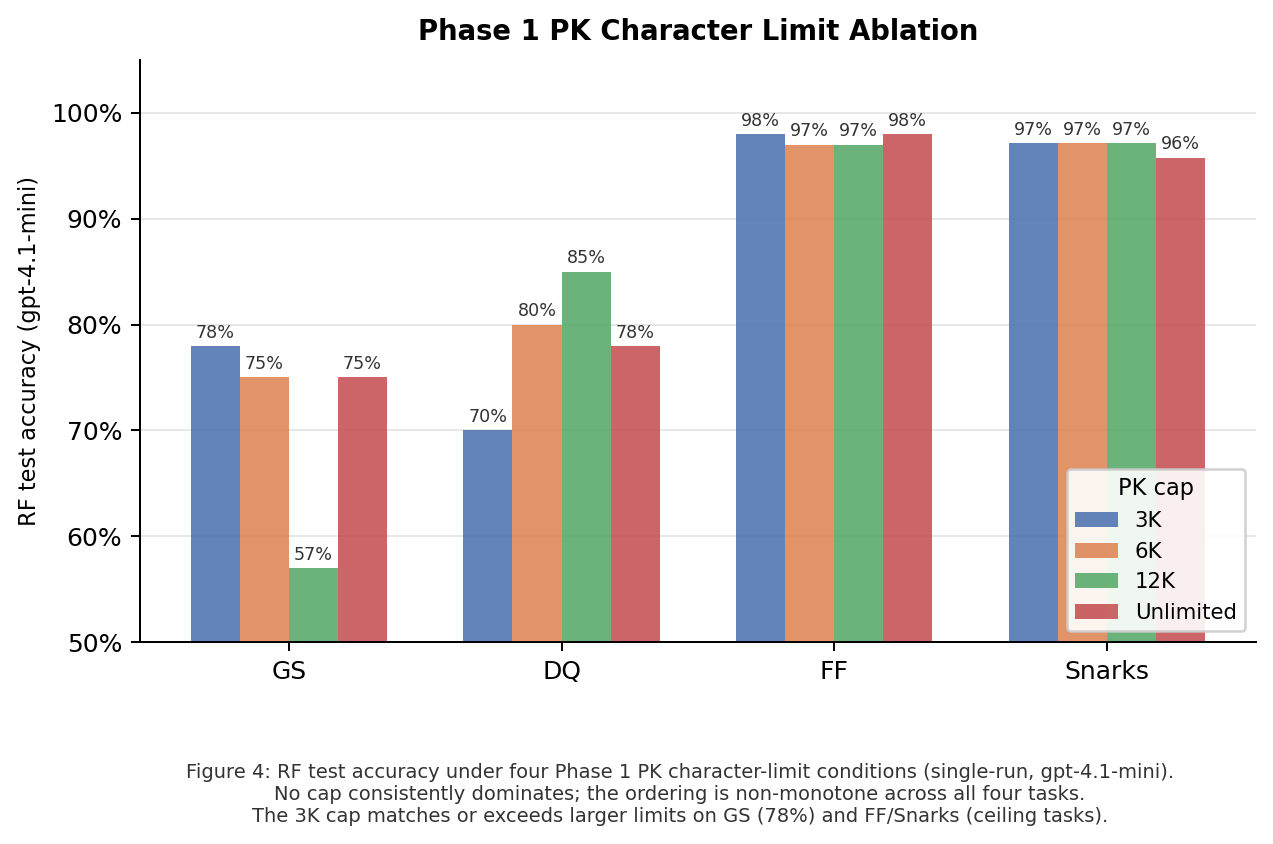
\includegraphics[width=\linewidth]{fig4_pk_size_ablation.png}
  \caption{Phase~1 PK character limit ablation---RF test accuracy (single-run). The ordering
    is non-monotone; no cap consistently outperforms.}
  \label{fig:pk_size}
\end{figure}

\subsection{Phase~2 best-of-$N$ case study selection}

The best-of-$N$ design loosens the acceptance gate and retains the top-$N$ case studies by
fix\_rate.
Table~\ref{tab:cs_ablation} and Figure~\ref{fig:cs_ablation} report RF test accuracy.
The key observation is a test-ordering reversal on GS: unlimited wins at test time
($78\%$) while best-of-3 led during training ($89.3\%$), illustrating the risk of using
train-accuracy metrics to select the case study count.
All other differences are within noise.

\begin{table}[h]
  \caption{Phase~2 case study count ablation---RF test accuracy on gpt-4.1-mini (single-run).
    ``---'' indicates Snarks had no pool excess under the unlimited condition.}
  \label{tab:cs_ablation}
  \centering
  \smallskip
  \begin{tabular}{lrrrr}
    \toprule
    \textbf{Task}
      & \textbf{Unlimited}
      & \textbf{Best-of-1}
      & \textbf{Best-of-3}
      & \textbf{Best CS (pool)} \\
    \midrule
    GS     & \textbf{78.0\%} & 69.0\% & 74.0\% & pool\,=\,4, best\,=\,100\% \\
    FF     & \textbf{97.0\%} & \textbf{97.0\%} & \textbf{97.0\%} & pool\,=\,5, best\,=\,50\%  \\
    Snarks & \textbf{97.2\%} & \textbf{97.2\%} & \textbf{97.2\%} & ---                        \\
    DQ     & \textbf{88.0\%} & \textbf{88.0\%} & 79.0\%          & pool\,=\,4, best\,=\,57\%  \\
    \bottomrule
  \end{tabular}
\end{table}

\begin{figure}[h]
  \centering
  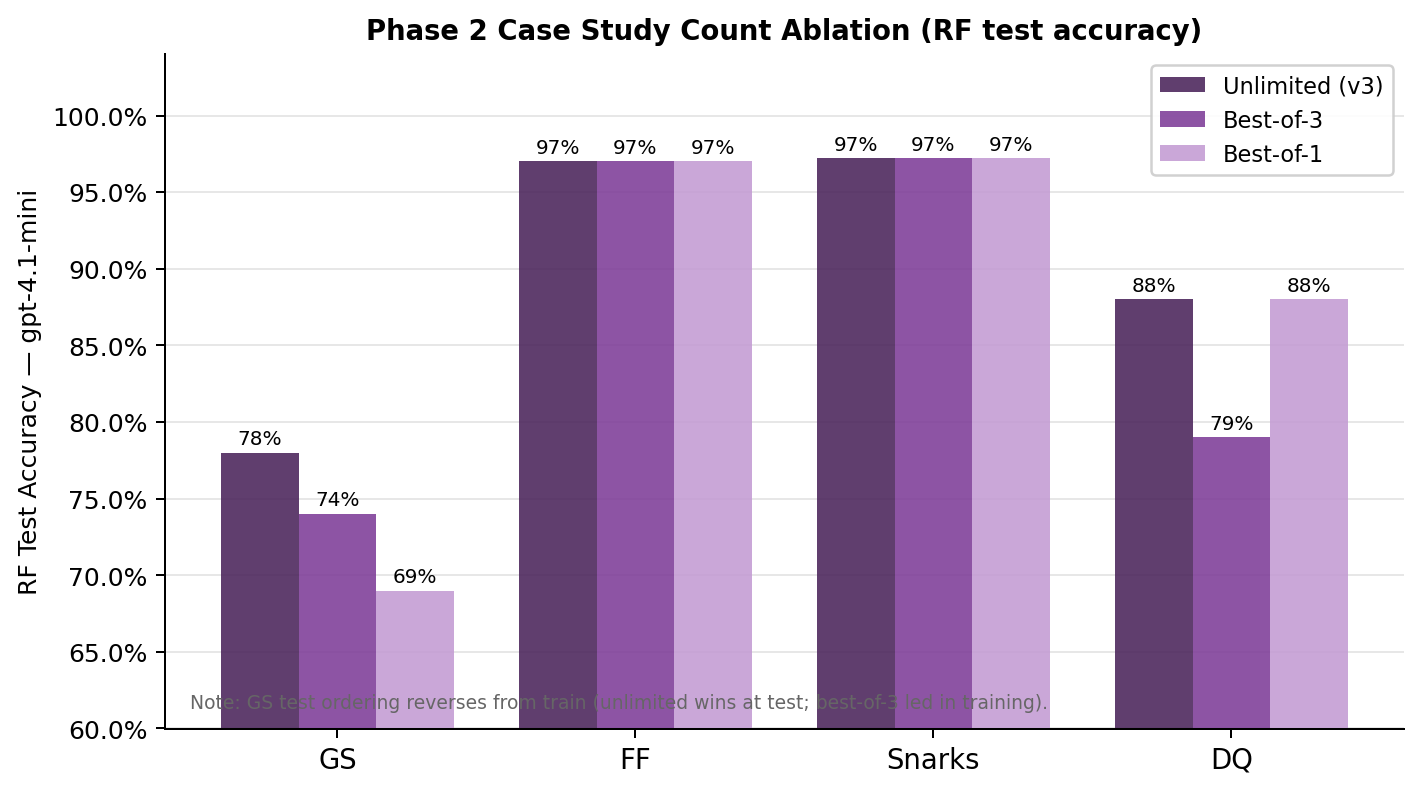
\includegraphics[width=0.85\linewidth]{fig3_phase2_cs_ablation.png}
  \caption{Phase~2 case study count ablation---RF test accuracy (single-run). GS test
    ordering reverses from train: unlimited wins. DQ shows best-of-3 performing worst.
    FF and Snarks are at ceiling across all conditions.}
  \label{fig:cs_ablation}
\end{figure}

\section{Causal Judgement: Cross-Seed Case Study Inventory}
\label{sec:cj_casestudies}

The main text (Section~\ref{sec:overfitting}) shows the single CJ case study from v3 seed~1,
which closely paraphrases a specific training item's oracle reasoning (Listing~\ref{lst:cj_cs}).
Table~\ref{tab:cj_casestudies} lists all case studies generated across seeds~1--3 of the
standard oracle-enabled v3 pipeline.
The key observation is that seeds~2 and 3 do \emph{not} exhibit the same oracle-derived
specificity as seed~1: they produce structurally formatted ACTIVATE~IF case studies rather
than free-form narratives, and none directly paraphrase a training item.
Nevertheless, \emph{all three seeds produce case studies that hurt evaluation accuracy}
(v3 full CJ non-train mean = 64.9--70.5\% vs CS-ICL CJ = 72.4\%), which implicates the
\emph{heterogeneous failure distribution} co-explanation: even structurally general case studies
cannot cover 35 training failures spanning 6+ causal sub-types.
Notably, seeds~2 and 3 converge on joint-AND causation and overdetermination patterns,
missing norm violations, timing effects, intentionality judgements, and prevention chains
entirely.

\begin{table}[h]
  \caption{CJ case studies generated across all three v3 pipeline seeds.
    Seed~1: 1 oracle-contaminated case study (free-form narrative, garden fertilizer paraphrase).
    Seeds 2--3: multiple structurally formatted case studies addressing joint-causation and
    redundancy patterns.
    All three seeds produce case studies that reduce transfer accuracy relative to CS-ICL,
    implicating both oracle contamination (seed~1) and failure-distribution heterogeneity
    (seeds 2--3) as contributing factors.}
  \label{tab:cj_casestudies}
  \centering
  \smallskip
  \begin{tabular}{p{0.5cm} p{5.2cm} p{5.0cm}}
    \toprule
    \textbf{Seed} & \textbf{Case study title / pattern} & \textbf{Observation} \\
    \midrule
    1 &
      \textit{Joint causes (logical AND): garden fertilizers} &
      Oracle-contaminated: free-form narrative paraphrasing one training item's gold
      chain-of-thought; encodes one idiosyncratic joint-AND scenario. \\
    \addlinespace
    2 &
      \textit{Overlapping Contributors with Non-Intersecting Effects}
      (joint-AND causation) &
      \multirow{3}{5.0cm}{Three structured ACTIVATE~IF case studies, all addressing the
      joint-AND / combined-harm pattern from different angles.
      No oracle paraphrase; ACTIVATE~IF conditions are abstract.
      Covers only one causal sub-type; misses norm violations, timing effects, and
      intentionality judgements.} \\
    2 & \textit{Joint Necessary Actions Without Individual Effect} & \\
    2 & \textit{Joint Harm Only from Combined Actions} & \\
    \addlinespace
    3 &
      \textit{Redundant Contributors in Joint Outcomes} (overdetermination)
      &
      \multirow{4}{5.0cm}{Four structured case studies spanning overdetermination,
      maintaining a sufficient condition, and compliance with instructions.
      More diverse than seed~2, but still omits norm violations, prevention chains,
      and intentionality sub-types. Two redundancy case studies are near-duplicates,
      paralleling the FF redundancy noted in Section~2.3---a recurring weakness of greedy
      partition search.} \\
    3 & \textit{Overdetermination with Redundant Contributors} & \\
    3 & \textit{Causation by Maintaining a Sufficient Condition} & \\
    3 & \textit{Causation by Complying with Essential Instructions} & \\
    \bottomrule
  \end{tabular}
\end{table}

\bibliographystyle{plainnat}
\bibliography{references}

\end{document}
